\begin{figure}[H]
    \centering
    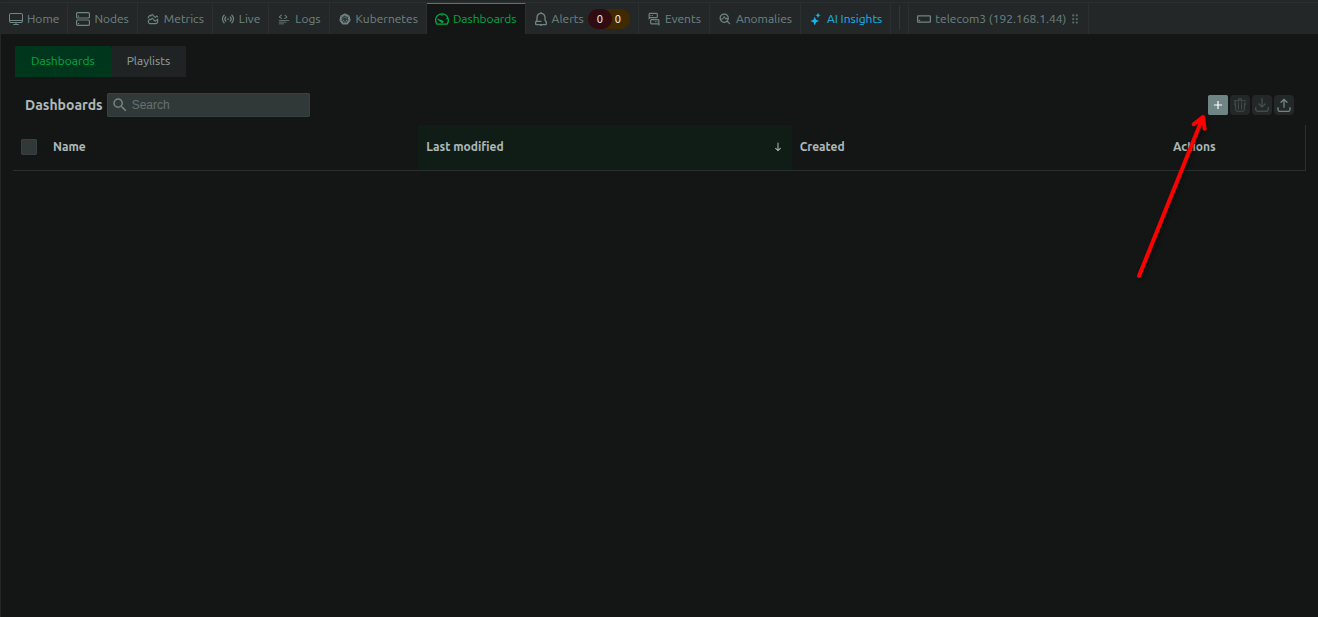
\includegraphics[scale= 0.4]{Pictures/7/5/1.png}
    \caption{Nuevo \textit{Dashboard}}
    \label{CON1}
\end{figure}

\begin{figure}[H]
    \centering
    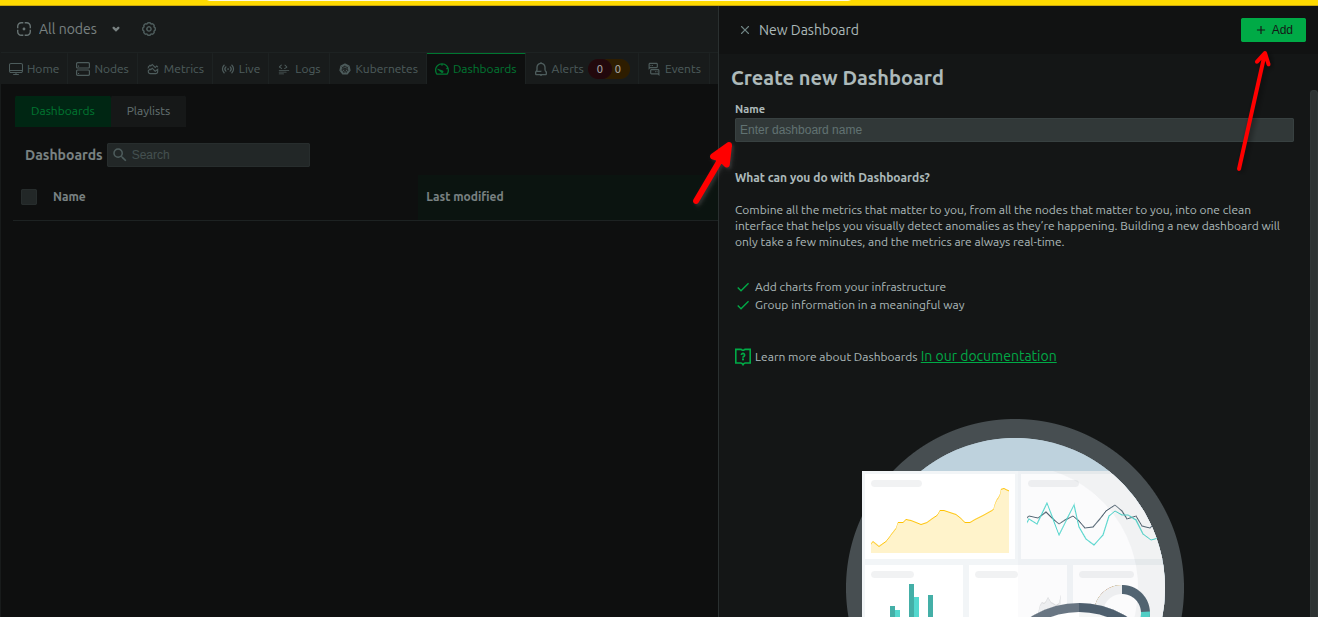
\includegraphics[scale= 0.4]{Pictures/7/5/2.png}
    \caption{Se le coloca nombre y \textit{Add}}
    \label{CON1}
\end{figure}


\begin{figure}[H]
    \centering
    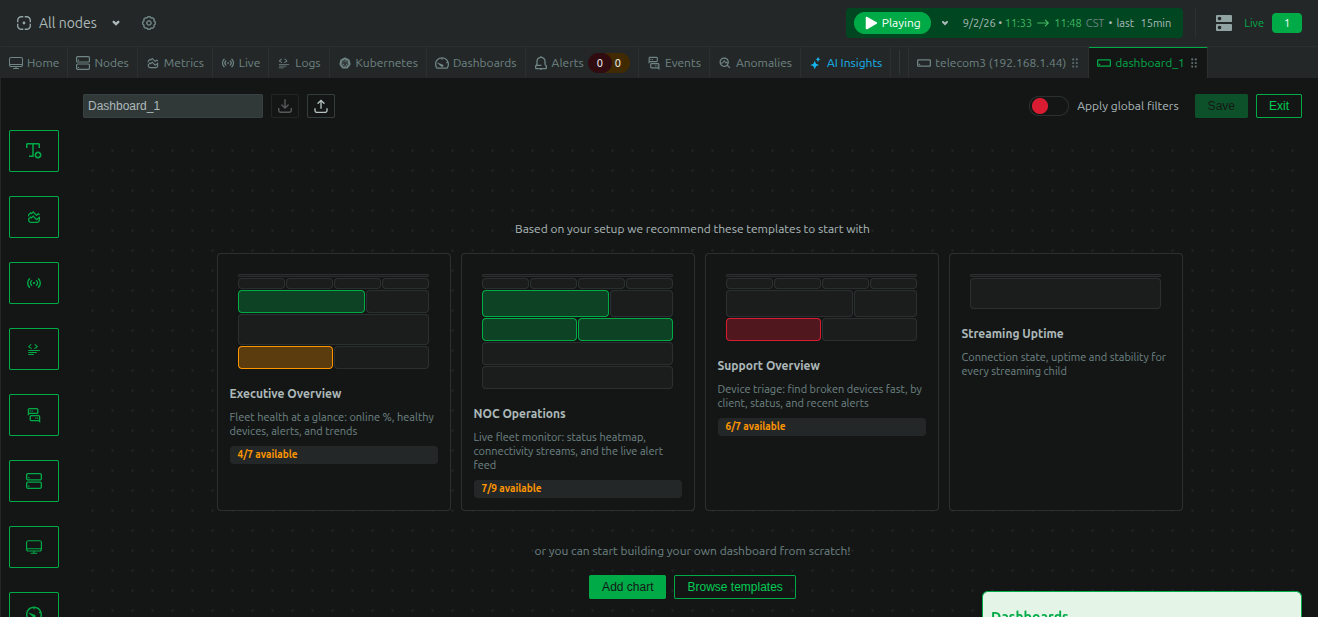
\includegraphics[scale= 0.4]{Pictures/7/5/3.png}
    \caption{Se pueden hacer nuevos \textit{templates} o diseñar uno desde 0}
    \label{CON1}
\end{figure}

\begin{figure}[H]
    \centering
    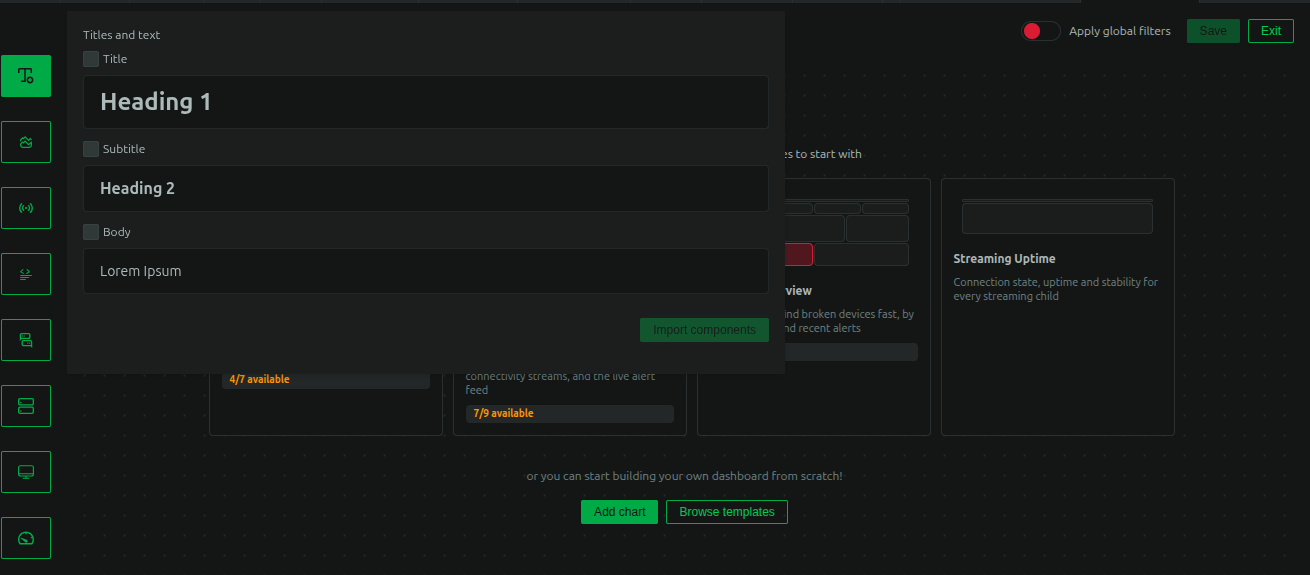
\includegraphics[scale= 0.4]{Pictures/7/5/4.png}
    \caption{\textit{Titles and text}}
    \label{CON1}
\end{figure}

\begin{figure}[H]
    \centering
    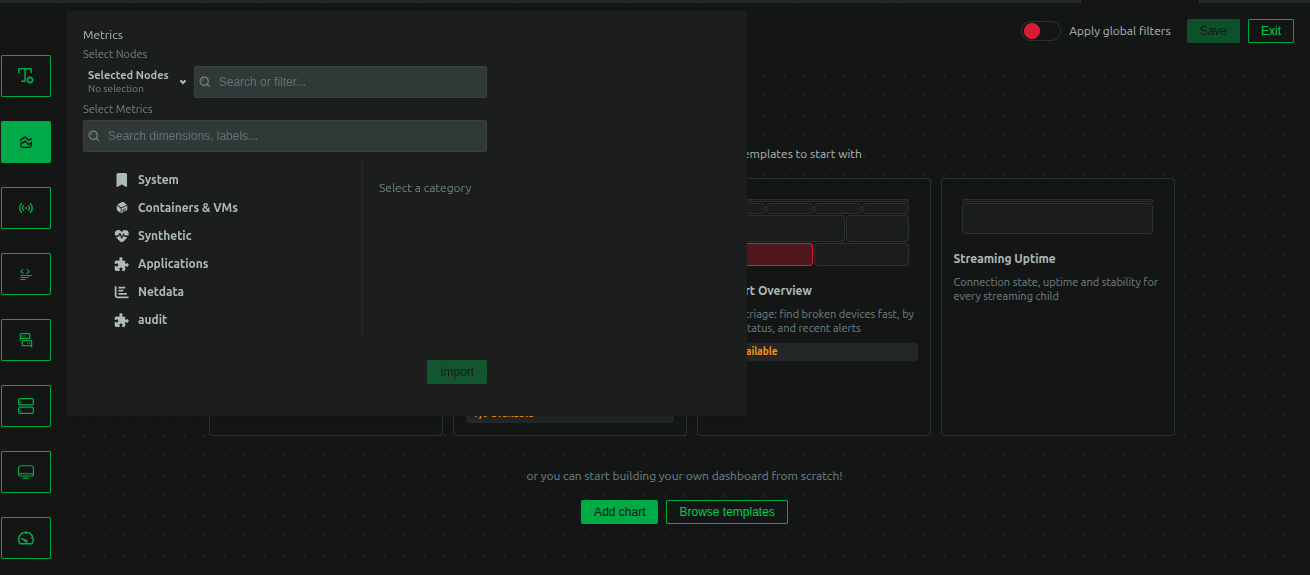
\includegraphics[scale= 0.4]{Pictures/7/5/5.png}
    \caption{\textit{Metrics}}
    \label{CON1}
\end{figure}


\begin{figure}[H]
    \centering
    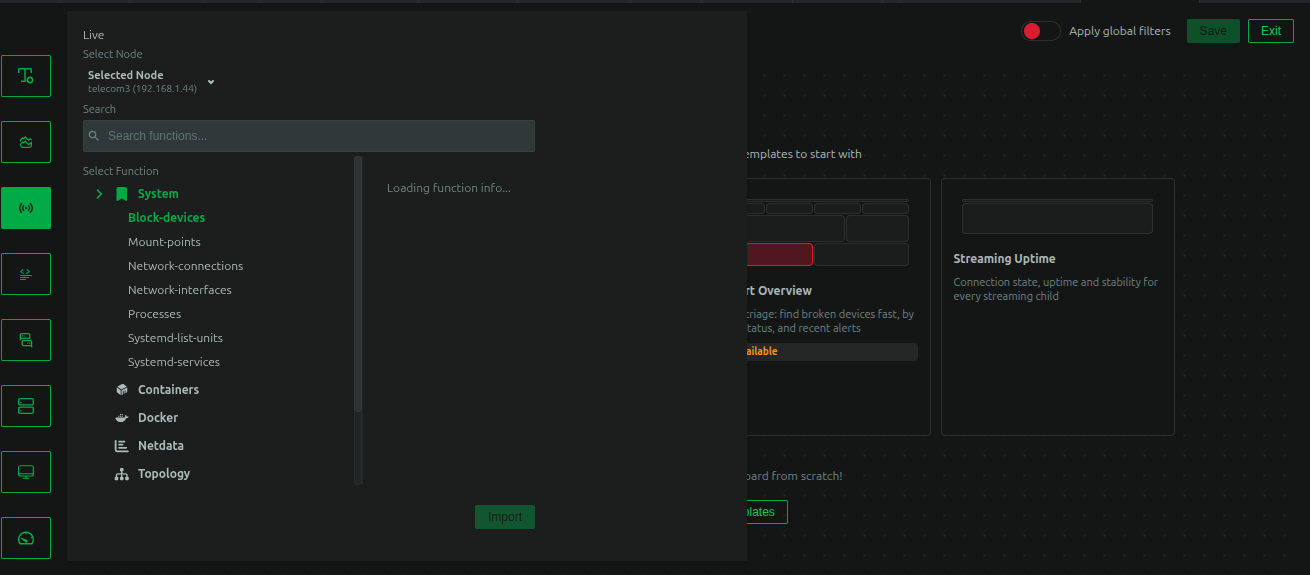
\includegraphics[scale= 0.4]{Pictures/7/5/6.png}
    \caption{\textit{Live}}
    \label{CON1}
\end{figure}

\begin{figure}[H]
    \centering
    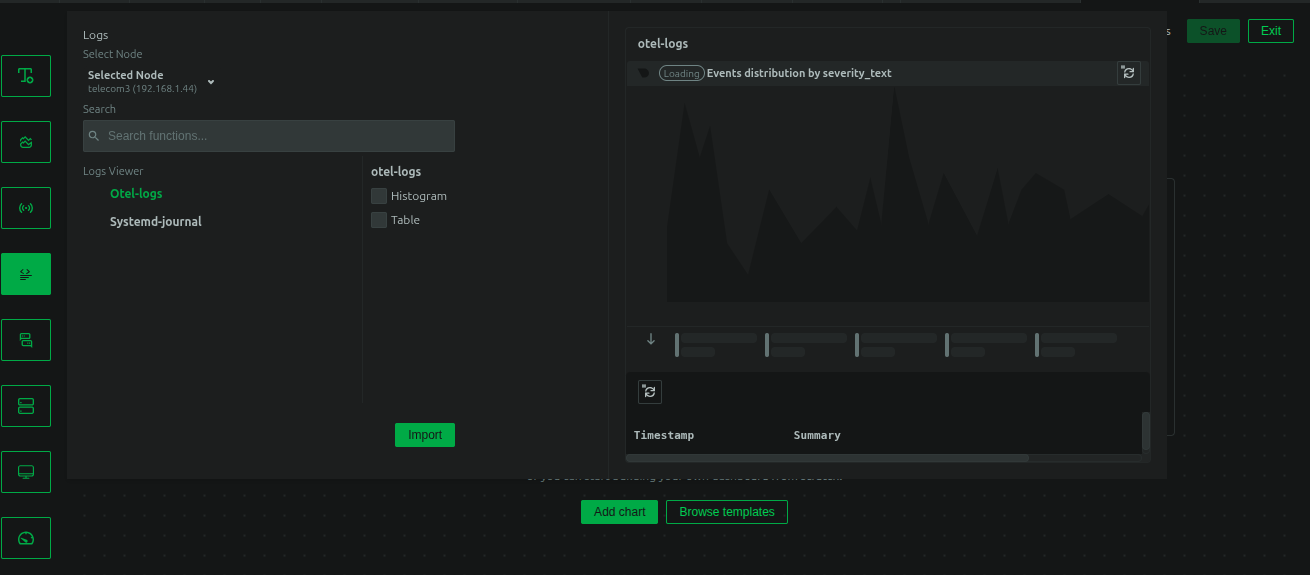
\includegraphics[scale= 0.4]{Pictures/7/5/7.png}
    \caption{\textit{Logs}}
    \label{CON1}
\end{figure}

\begin{figure}[H]
    \centering
    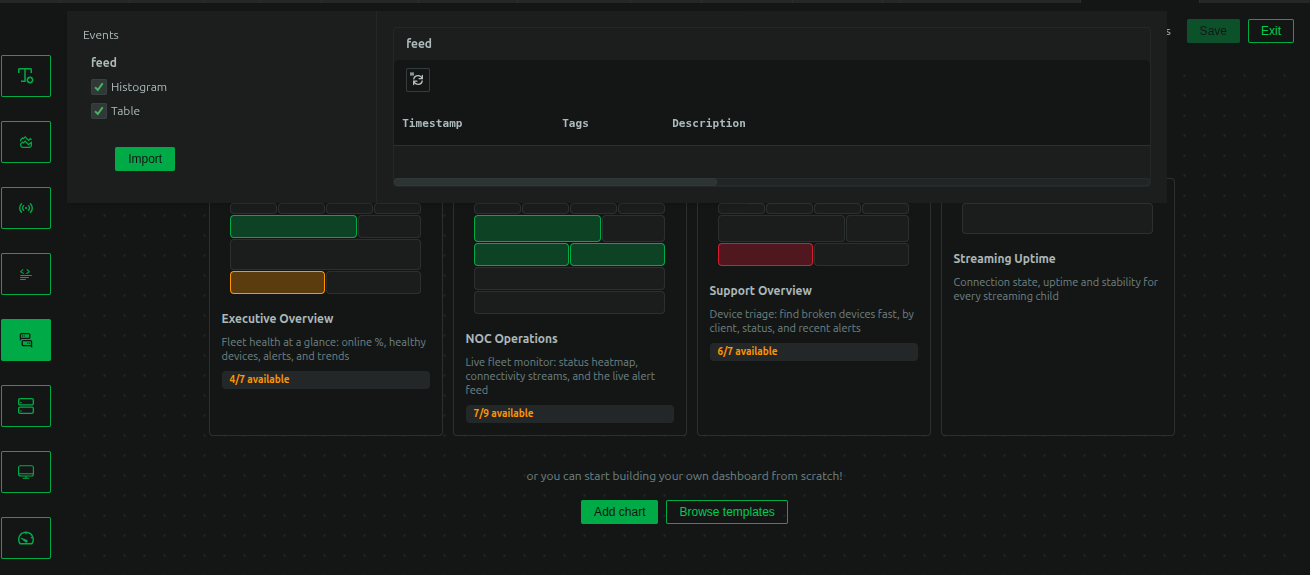
\includegraphics[scale= 0.4]{Pictures/7/5/8.png}
    \caption{\textit{Events}}
    \label{CON1}
\end{figure}


\begin{figure}[H]
    \centering
    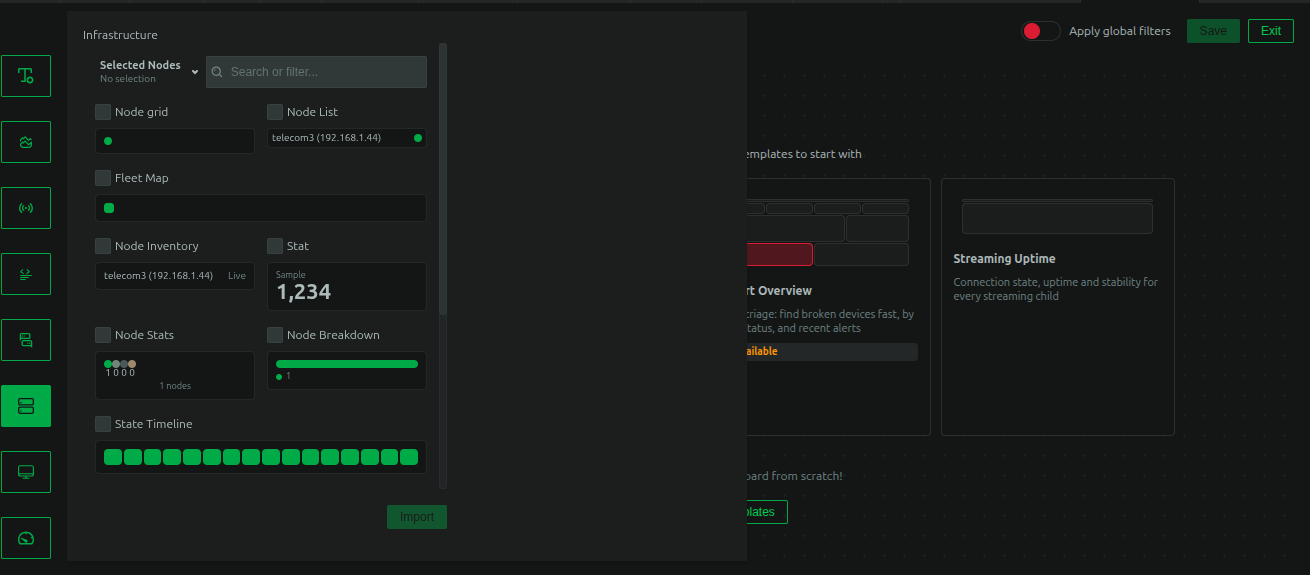
\includegraphics[scale= 0.4]{Pictures/7/5/9.png}
    \caption{\textit{Infrastructure}}
    \label{CON1}
\end{figure}

\begin{figure}[H]
    \centering
    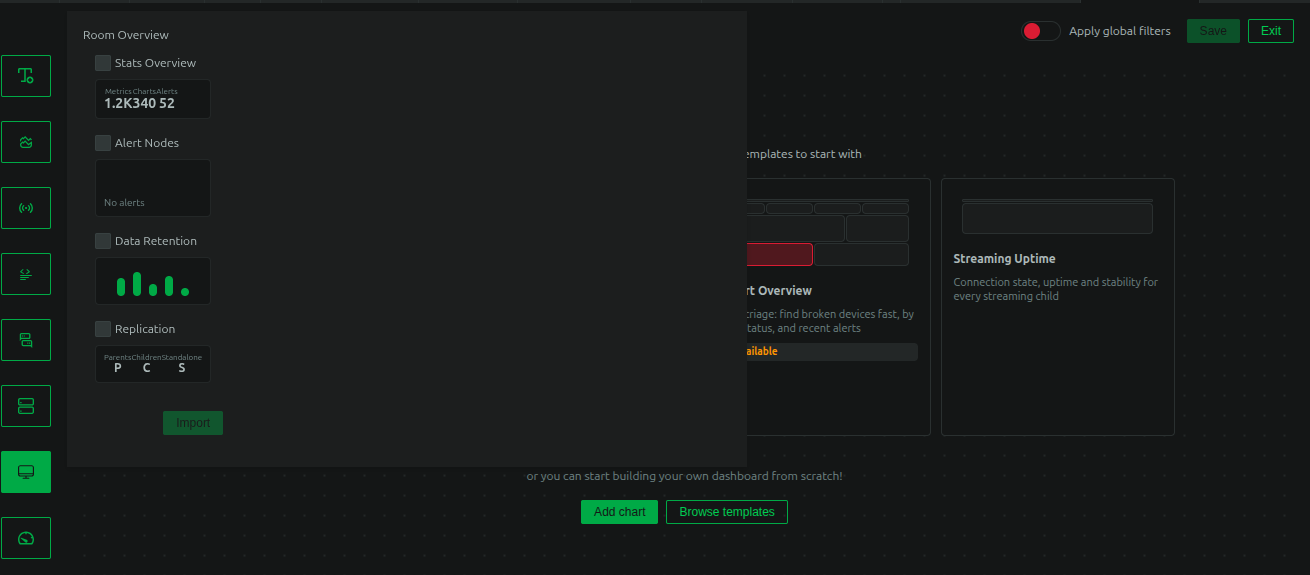
\includegraphics[scale= 0.4]{Pictures/7/5/10.png}
    \caption{\textit{Room Overview}}
    \label{CON1}
\end{figure}

\begin{figure}[H]
    \centering
    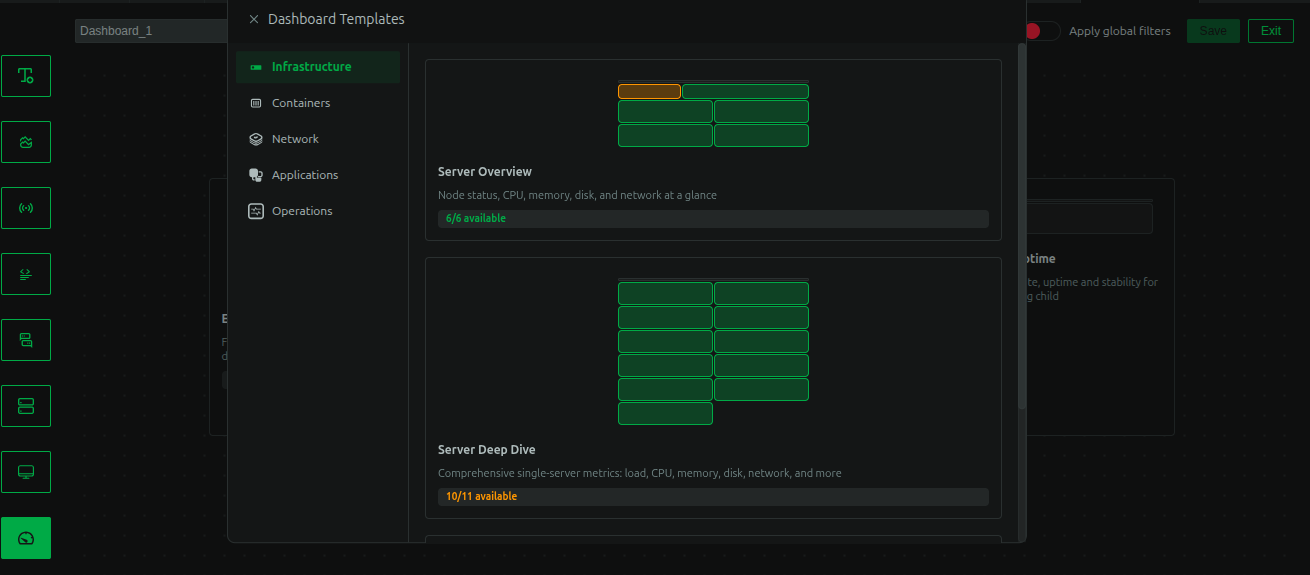
\includegraphics[scale= 0.4]{Pictures/7/5/11.png}
    \caption{\textit{Dashboard Templates}}
    \label{CON1}
\end{figure}
